\subsection{802.11 Overview}
\subsubsection{Frame Types}
There are three frame categories defined in the 802.11 standard \cite{research:80211_standard}: management, control and data. These types are further split into subtypes which determines which frame is being sent/received. For the purpose of performing an association sequence, we are interested in frames from the management category. The table below details these frames, along with their type, subtype and originating source, in order for us to successfully filter packets in wireshark to capture the sequence.

\begin{table}[h!]
\begin{center}
	\begin{tabular}{| c | c |}
		\hline
		\textbf{Type} & \textbf{Description} \\ \hline
		0x00 & Management \\ \hline
		0x01 & Control \\ \hline
		0x02 & Data \\ \hline
	\end{tabular}
	
\end{center}
\end{table}
\begin{table}[h!]
\begin{center}
	\begin{tabular}{| c | c | c | c |}
		\hline
		\textbf{Type} & \textbf{Subtype} &  \textbf{Description} &  \textbf{Source} \\ \hline
		0x00 & 0x40 & Probe Request & Station \\ \hline
		0x00 & 0x50 & Probe Response & Access Point \\ \hline
		0x00 & 0xb0 & Authentication & Station \\ \hline
		0x00 & 0xb0 & Authentication & Access Point \\ \hline
		0x00 & 0x00 & Association Request & Station \\ \hline
		0x00 & 0x10 & Association Request & Access Point \\ \hline
	\end{tabular}
\end{center}
\end{table}

One of the key issues with the 802.11 standard is that management frames are not encrypted. This is what a large majority of attacks take advantage of by way of a gateway to further attacks, as detailed in a later section.

\clearpage
\subsubsection{General Frame Structure}
Figure \ref{fig:framestructure} below details the contents and size of each field in the general frame structure for an 802.11 packet. A description of the contents are detailed table \ref{table:framefields}, with the frame control segment's fields being detailed in table \ref{table:framecontrol}.

\begin{figure}[h!]
\centering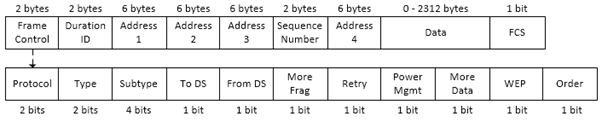
\includegraphics[width=\linewidth]{research/80211/figures/framestructure.png}
\caption{General frame structure.}
\label{fig:framestructure}
\end{figure}

	\begin{table}[!h]
\begin{center}
	\begin{tabular}{| c |  p{5cm} |}
		\hline
		\textbf{Field} & \textbf{Description} \\ \hline
		Frame Control & Detailed in table \ref{table:framecontrol} on page \pageref{table:framecontrol}.\\ \hline
		Duration ID & Control \\ \hline
		Addresses & Four addresses can be present.  They show the source and destination addresses, and may also give the BSSID, transmitter, and receiver address.  \\ \hline
		Sequence Number & This allows stations to prevent duplicated frames by keeping track of the current sequence number. \\ \hline
		Data & This is the body of the frame. It can contain 2048 bytes with a 256 byte upper layer header when sent by an application. \\ \hline
		FCS & The CRC \cite{research:crc_wiki} of the frame. \\ \hline
	\end{tabular}
	\caption{General frame structure fields.}
	\label{table:framefields}
\end{center}
	\end{table}

\begin{table}[!h]
\begin{center}
	\begin{tabular}{ | c |  p{5cm} | }
 		\hline
		\textbf{Protocol} & Identifies the version of the 802.11 MAC protocol. \\ \hline
		\textbf{Type} & Identifies the group of the frame. \\ \hline
		\textbf{Subtype} & Identifies the type of frame in the group; determines what should be present in the rest of the frame. \\ \hline
		\textbf{To DS} & Set when the frame originates from a station. \\ \hline
		\textbf{From DS} & Set when the frame originates from the access point. \\ \hline
		\textbf{More Fragment} & Indicates whether this frame is the last in a set of packets. \\ \hline
		\textbf{Retry} & Determines whether this frame is a retransmission. \\ \hline
		\textbf{Power Management} & A mobile station gives it’s power management state: 0 is active mode, 1  means the station will enter the power management mode. \\ \hline
		\textbf{More Data} & Determines whether an access point has cached data for a station. Used during roaming when crossing boundaries between BSSs. \\ \hline
		\textbf{WEP} & Determines whether the frame body has been encrypted using the WEP \cite{research:wep} algorithm.  \\ \hline
		\textbf{Order} & Identifies whether the frames are ordered or not. \\ \hline
	\end{tabular}
		\caption{Frame Control fields.}
		\label{table:framecontrol}
\end{center}
\end{table}
\clearpage
\subsubsection{Determining 802.11 Open Association Sequence}
In order to create a fake access point for devices that are broadcasting probe requests for previously connected open networks, the application needs to follow the same sequence that a real access point would when responding to probe requests. I need to be able to discern which flags are to be set, and the values to give, in each frame in order for the smartphone to be able to connect, and also find out where the authentication type is revealed. 

To watch the association sequence happen in real-time, and determine when in the sequence the authentication type is given, I needed to set up a simple wireless network, and have a wireless adaptor running in monitor mode filtering packets as a smartphone associates with the access point. This method would allow me to utilize wireshark to inspect other elements of the sequence that aren’t necessarily detailed in online sources, such as the various flags set in each frame.

The first step in the process is setting up Backtrack with the Alfa wireless adaptor plugged in, and creating a monitor interface on wlan0 using airmon-ng:

\begin{figure}[h!]
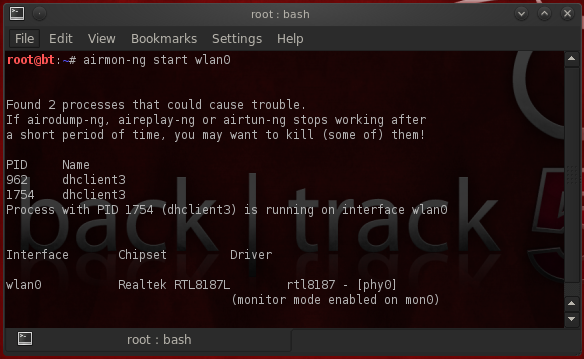
\includegraphics[width=\linewidth]{research/80211/figures/bt1.png}
\caption{Start monitor interface.}
\label{research:80211:bt1}
\end{figure}

This would allow me to capture traffic as it passes by in wireshark by sniffing on mon0, and filter it down to the frames that I am interested in. To get a first hand look at the sequence I setup the wireless router, gave it a unique SSID, left encryption set to open, noted down it’s mac address, and setup a filter on wireshark that would only report packets with a source address of my iPhone and broadcast as the destination. With this filter in place I could look at the probe request frames sent from my phone as it searched for the access point. This is the start of the association sequence we’re after. It’s from these requests we’ll forge frames to convince the device we are the real AP.

\begin{figure}[h!]
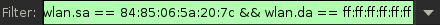
\includegraphics[width=\linewidth]{research/80211/figures/bt2.png}
\caption{Wireshark filter.}
\label{research:80211:bt2}
\end{figure}

\begin{figure}[h!]
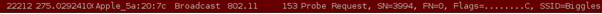
\includegraphics[width=\linewidth]{research/80211/figures/bt3.png}
\caption{Wireshark captured probe request.}
\label{research:80211:bt3}
\end{figure}

\begin{figure}[h!]
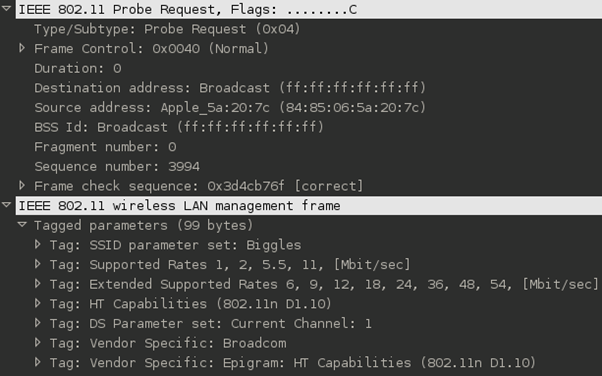
\includegraphics[width=\linewidth]{research/80211/figures/bt4.png}
\caption{Probe request contents.}
\label{research:80211:bt4}
\end{figure}
\newpage
This revealed the probe request subtype that the application would need to search incoming packet headers for to determine whether it would need to kick off the sequence to create a fake access point.

The next step was to filter for probe response frames so I could understand how an access point reacts to receiving a probe request, primarily determining which information element fields to set in the management frame.

\begin{figure}[h!]
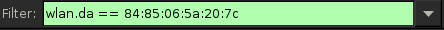
\includegraphics[width=\linewidth]{research/80211/figures/bt5.png}
\caption{Wireshark destination MAC address filter.}
\label{research:80211:bt5}
\end{figure}

This revealed the response the Netgear router has sent my phone.

\begin{figure}[h!]
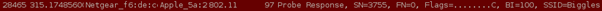
\includegraphics[width=\linewidth]{research/80211/figures/bt6.png}
\caption{Probe response frame}
\label{research:80211:bt6}
\end{figure}
\newpage
The probe response frame shows which IE fields are required in the management header, namely the SSID (which will be a mirror of the one in the probe request), the supported rates, channel information and ERP information. 

\begin{figure}[h!]
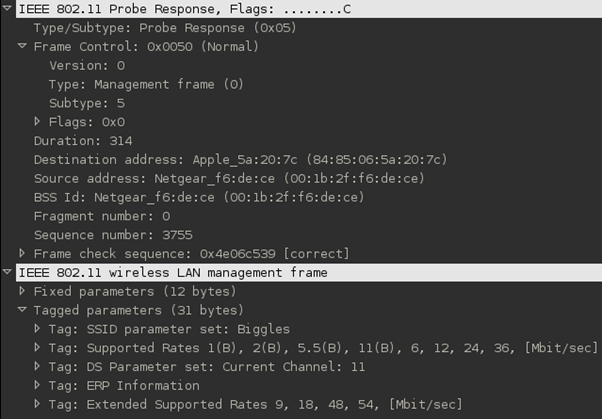
\includegraphics[width=\linewidth]{research/80211/figures/bt65.png}
\caption{Probe response contents.}
\label{research:80211:bt65}
\end{figure}

The next step in the sequence that we are interested in is the association. This frame gives us information related to the encryption standard that the network the station is trying to connect to uses. Figure \ref{research:80211:bt7} shows the request sent from my phone to the Netgear router, and figure \ref{research:80211:bt8} shows the contents.

\begin{figure}[h!]
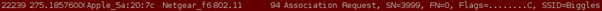
\includegraphics[width=\linewidth]{research/80211/figures/bt7.png}
\caption{Association request.}
\label{research:80211:bt7}
\end{figure}
\clearpage
\begin{figure}[h!]
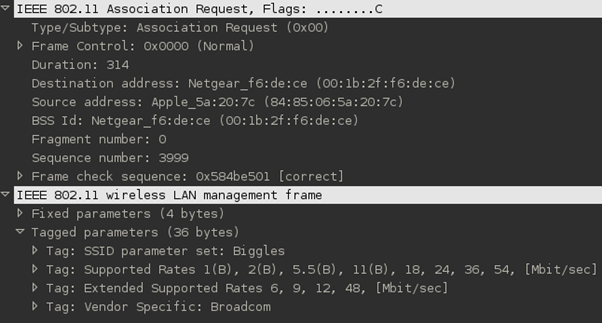
\includegraphics[width=\linewidth]{research/80211/figures/bt8.png}
\caption{Association request frame contents.}
\label{research:80211:bt8}
\end{figure}

This is the point I need to get to programmatically before starting the fake access point, as I can ensure that the device is indeed looking for a network with open authentication, thus eliminating any unnecessary connection attempts.